\chapter{Measurements}
\section{Overview}
The measurements were performed in an open filed with a \textit{DJI Mavic Pro} drone.
A measurement location with low ambient noise was chosen.
However, a nearby farm was sometimes audible in the recordings.

\section{Stationary Drone}
In the stationary drone test, the drone flew to different points,
where it then stayed still.
For the test five points in different directions were chosen.
Table \ref{meas:tabP} shows these five points.
These points were measured using the \acrshort{gps} of the drone
so their position are not known with great precision.
At each of the five points the array was tested with five
different arm angles.

\begin{table}[h]
	\centering
	\begin{tabular}{ |c"c|c|c| }
		\hline
		                        & \makecell{$\phi_s$} &
		\makecell{$\theta_s$}   &
		\makecell{$r_s$}                                \\
		\thickhline
		$\bm{P_1}$              &
		\makecell{$-120^\circ$} &
		\makecell{$70^\circ$}   &
		\makecell{$31$\,m}                              \\
		\hline
		$\bm{P_2}$              &
		\makecell{$-158^\circ$} &
		\makecell{$50^\circ$}   &
		\makecell{$17$\,m}                              \\
		\hline
		$\bm{P_3}$              &
		\makecell{$-158^\circ$} &
		\makecell{$25^\circ$}   &
		\makecell{$32$\,m}                              \\
		\hline
		$\bm{P_4}$              &
		\makecell{$-158^\circ$} &
		\makecell{$15^\circ$}   &
		\makecell{$52$\,m}                              \\
		\hline
		$\bm{P_5}$              &
		\makecell{$0^\circ$}    &
		\makecell{$0^\circ$}    &
		\makecell{$50$\,m}                              \\
		\hline
	\end{tabular}
	\caption{Postions of the test points.}
	\label{meas:tabP}
\end{table}

The measurements include the calculated \acrshort{doa} and the two metrics introduced
in section \ref{sec:metrics}.
Tables \ref{meas:tabPhi} and \ref{meas:tabtheta} show the signed error
for the two angles $\phi$ and $\theta$.
The measurement of $\phi$ is relatively independent of the array arm angle.
However for positions with a high $\theta_s$ the error in $\theta$ increases
when the arm angle increases.
Since this was not the case in the simulation, it is suspected that
these errors come from physical effects of the sound waves in the array
and the directionality of the used microphones.

\begin{table}[ht]
	\centering
	\begin{tabular}{ |P{1.8cm}"l|l|l|l|l | }
		\hline
		Arm angle             & \makecell{$\bm{P}_1$} &
		\makecell{$\bm{P}_2$} &
		\makecell{$\bm{P}_3$} &
		\makecell{$\bm{P}_4$} &
		\makecell{$\bm{P}_5$}                           \\
		\thickhline
		$0^\circ$             &
		$-2^\circ$            &
		\makecell{$+5^\circ$} &
		\makecell{$+2^\circ$} &
		\makecell{$+3^\circ$} &
		\makecell{$0^\circ$}                            \\
		\hline
		$15^\circ$            &
		\makecell{$-2^\circ$} &
		\makecell{$-1^\circ$} &
		\makecell{$+0^\circ$} &
		\makecell{$+2^\circ$} &
		\makecell{$+0^\circ$}                           \\
		\hline
		$30^\circ$            &
		\makecell{$-2^\circ$} &
		\makecell{$+6^\circ$} &
		\makecell{$+1^\circ$} &
		\makecell{$+4^\circ$} &
		\makecell{$+0^\circ$}                           \\
		\hline
		$45^\circ$            &
		\makecell{$-1^\circ$} &
		\makecell{$+6^\circ$} &
		\makecell{$+2^\circ$} &
		\makecell{$+5^\circ$} &
		\makecell{$+0^\circ$}                           \\
		\hline
		$60^\circ$            &
		\makecell{$-2^\circ$} &
		\makecell{$+6^\circ$} &
		\makecell{$+4^\circ$} &
		N/A                   &
		N/A                                             \\
		\hline
	\end{tabular}
	\caption{Signed error in $\phi$.
		The errors for $\bm{P}_5$ are 0 due to its indefiniteness when $\theta = 0^\circ$.}
	\label{meas:tabPhi}
\end{table}

\begin{table}[ht]
	\centering
	\begin{tabular}{ |P{1.8cm}"l|l|l|l|l | }
		\hline
		Arm angle              & \makecell{$\bm{P}_1$} &
		\makecell{$\bm{P}_2$}  &
		\makecell{$\bm{P}_3$}  &
		\makecell{$\bm{P}_4$}  &
		\makecell{$\bm{P}_5$}                            \\
		\thickhline
		$0^\circ$              &
		\makecell{$+2^\circ$}  &
		\makecell{$+5^\circ$}  &
		\makecell{$+0^\circ$}  &
		\makecell{$+0^\circ$}  &
		\makecell{$+1^\circ$}                            \\
		\hline
		$15^\circ$             &
		\makecell{$+5^\circ$}  &
		\makecell{$+5^\circ$}  &
		\makecell{$+0^\circ$}  &
		\makecell{$+0^\circ$}  &
		\makecell{$+1^\circ$}                            \\
		\hline
		$30^\circ$             &
		\makecell{$+10^\circ$} &
		\makecell{$+9^\circ$}  &
		\makecell{$+1^\circ$}  &
		\makecell{$+0^\circ$}  &
		\makecell{$+1^\circ$}                            \\
		\hline
		$45^\circ$             &
		\makecell{$+20^\circ$} &
		\makecell{$+10^\circ$} &
		\makecell{$+1^\circ$}  &
		\makecell{$+0^\circ$}  &
		\makecell{$+1^\circ$}                            \\
		\hline
		$60^\circ$             &
		\makecell{$+20^\circ$} &
		\makecell{$+11^\circ$} &
		\makecell{$+2^\circ$}  &
		N/A                    &
		N/A                                              \\
		\hline
	\end{tabular}
	\caption{Signed error in $\theta$.}
	\label{meas:tabtheta}
\end{table}

The mainlobe areas from the measurements are as expected from the simulations.
It is however observed that the mainlobe area at $\bm{P}_1, \bm{P}_3$ and $\bm{P}_4$
is better when the arm is angled.
With the current measurements it can not be stated if this results from noise or
from other effects.

The \acrshort{pap} ratio is significantly lower than in the simulated cases.
Since the measurement was taken outdoors with background noise,
this is no surprise.
Nonetheless the \acrshort{pap} ratio follows similar trends when $\theta_s$ or the arm angle is changed.
\begin{table}[h]
	\centering
	\begin{tabular}{ |P{1.8cm}"P{2cm}|P{2cm}|P{2cm}|P{2cm}|P{2cm} | }
		\hline
		Arm angle             & \makecell{$\bm{P}_1$} &
		\makecell{$\bm{P}_2$} &
		\makecell{$\bm{P}_3$} &
		\makecell{$\bm{P}_4$} &
		\makecell{$\bm{P}_5$}                           \\
		\thickhline
		$0^\circ$             &
		\makecell{$4.85\%$}   &
		\makecell{$4.37\%$}   &
		\makecell{$2.42\%$}   &
		\makecell{$2.90$\%}   &
		\makecell{$1.45\%$}                             \\
		\hline
		$15^\circ$            &
		\makecell{$4.24\%$}   &
		\makecell{$4.52\%$}   &
		\makecell{$2.01\%$}   &
		\makecell{$1.82\%$}   &
		\makecell{$2.00\%$}                             \\
		\hline
		$30^\circ$            &
		\makecell{$4.15\%$}   &
		\makecell{$6.71\%$}   &
		\makecell{$2.92\%$}   &
		\makecell{$2.30\%$}   &
		\makecell{$1.82\%$}                             \\
		\hline
		$45^\circ$            &
		\makecell{$4.10\%$}   &
		\makecell{$6.62\%$}   &
		\makecell{$4.62\%$}   &
		\makecell{$2.95\%$}   &
		\makecell{$2.31\%$}                             \\
		\hline
		$60^\circ$            &
		\makecell{$4.26\%$}   &
		\makecell{$6.76\%$}   &
		\makecell{$5.16\%$}   &
		N/A                   &
		N/A                                             \\
		\hline
	\end{tabular}
	\caption{Mainlobe area ratio at the testpoints.}
	\label{meas:tabarea}
\end{table}

\begin{table}[h]
	\centering
	\begin{tabular}{ |P{1.8cm}"P{2cm}|P{2cm}|P{2cm}|P{2cm}|P{2cm} | }
		\hline
		Arm angle             & \makecell{$\bm{P}_1$} &
		\makecell{$\bm{P}_2$} &
		\makecell{$\bm{P}_3$} &
		\makecell{$\bm{P}_4$} &
		\makecell{$\bm{P}_5$}                           \\
		\thickhline
		$0^\circ$             &
		\makecell{$7.17$}     &
		\makecell{$10.20$}    &
		\makecell{$12.23$}    &
		\makecell{$7.65$}     &
		\makecell{$16.82$}                              \\
		\hline
		$15^\circ$            &
		\makecell{$9.30$}     &
		\makecell{$9.95$}     &
		\makecell{$11.81$}    &
		\makecell{$13.94$}    &
		\makecell{$14.51$}                              \\
		\hline
		$30^\circ$            &
		\makecell{$9.45$}     &
		\makecell{$8.35$}     &
		\makecell{$10.61$}    &
		\makecell{$11.30$}    &
		\makecell{$13.45$}                              \\
		\hline
		$45^\circ$            &
		\makecell{$9.14$}     &
		\makecell{$7.98$}     &
		\makecell{$7.74$}     &
		\makecell{$8.26$}     &
		\makecell{$11.56$}                              \\
		\hline
		$60^\circ$            &
		\makecell{$9.68$}     &
		\makecell{$8.34$}     &
		\makecell{$5.16$}     &
		N/A                   &
		N/A                                             \\
		\hline
	\end{tabular}
	\caption{PAP ratio at the testpoints.}
	\label{meas:tabPap}
\end{table}

\newpage
\section{Moving Drone Test}
Making a verifiable test for a flying drone was not possible due to
a lack of time.
To test the localization and tracking of a flying drone qualitative
tests were performed.
For the test the drone flew along paths in the test environment.
Ideally the track created by the drone is parallel to these paths.
To check the $\theta$ angle, the same track was flew in different height.
A comparison of two such flights are shown in Figure \ref{meas:fig:west east}.
In Figure \ref{meas:fig:west east high}, it is apparent that when the drone ascended by 10 meters,
the measured $\theta$ was lower than in Figure \ref{meas:fig:west east low}, as anticipated.

\begin{figure}[h]
	\centering
	\begin{subfigure}[t]{0.45\textwidth}
		\centering
		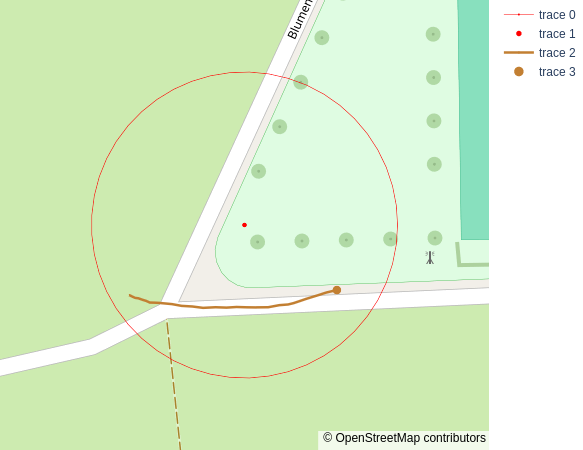
\includegraphics[width=\textwidth]{images/7_measurements/we_low.png}
		\caption{Drone flies in $40$\,m elevation}
		\label{meas:fig:west east low}
	\end{subfigure}
	\hfill
	\begin{subfigure}[t]{0.45\textwidth}
		\centering
		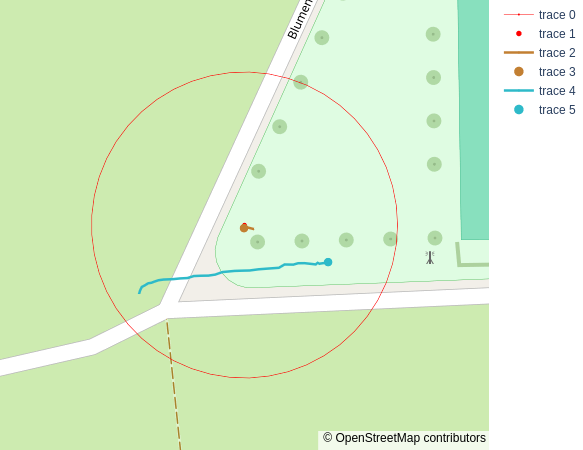
\includegraphics[width=\textwidth]{images/7_measurements/we_high.png}
		\caption{Drone flies in $50$\,m elevation}
		\label{meas:fig:west east high}
	\end{subfigure}
	\caption{Drone flying along the road from west to east in two different
		elevations.
		The distance between the red center point and the track is linearly
		dependent on $\theta$ whereas the angle between east and the track represents $\phi$.
		The thicker point right of the tracks shows the current tracker positions.}
	\label{meas:fig:west east}
\end{figure}

\section{Conclusion}
With these measurements it has been shown that the proposed microphone
array and sound source tracker are able
to localize and track flying drones.
To make better quantitative statements, more elaborate tests
would be needed.